%\documentclass[10pt]{beamer}
\documentclass[10pt, aspectratio=169]{beamer}

% MADRID THEME
%\usetheme{Madrid}
%\usecolortheme{whale}

\usetheme{metropolis}

\usepackage{amsmath}
\usepackage{amssymb}
\usepackage{amsfonts}
\usepackage{algorithmic}
\usepackage{tikz}
\usetikzlibrary{automata, positioning, arrows.meta, shapes.geometric}

\definecolor{verdeSalvia}{RGB}{112, 130, 114}  
\definecolor{grigioScuro}{RGB}{60, 64, 61}     
\definecolor{grigioSfondo}{RGB}{245, 246, 245} 
\definecolor{verdelime}{RGB}{154, 181, 16}
\definecolor{verdeOlivaScuro}{RGB}{75, 90, 76}

\setbeamercolor{structure}{fg=verdeSalvia}
\setbeamercolor{normal text}{fg=grigioScuro}
\setbeamercolor{alerted text}{fg=verdelime}
\setbeamercolor{block title}{bg=verdeSalvia, fg=white}
\setbeamercolor{block body}{bg=grigioSfondo, fg=grigioScuro}

% Configurazione degli elenchi puntati nello stile standard
\setbeamertemplate{enumerate items}[default]

\setbeamertemplate{enumerate items}[default]



%%%%%%%%%%%%%%%%%%%% DRAWINGs %%%%%%%%%%%%%%%%%%%%%%%%
% 1. FIXED: Larger triangle inside the Base circles
\tikzset{
        edgeLabel/.style={sloped, fill=grigioSfondo, inner sep=1.5pt, rounded corners=2pt}
    }
\newcommand{\bluebase}{\tikz[baseline=-0.5ex]{
    \node[circle, fill=blue!30, minimum size=9pt, inner sep=0pt] (c) {};
    \node[draw=grigioScuro, scale=0.6, regular polygon, regular polygon sides=3, fill=blue!60, inner sep=0pt, minimum size=7pt] at (c) {};
}}
\newcommand{\redbase}{\tikz[baseline=-0.5ex]{
    \node[circle, fill=red!30, minimum size=9pt, inner sep=0pt] (c) {};
    \node[draw=grigioScuro, scale=0.6, regular polygon, regular polygon sides=3, fill=red!70, inner sep=0pt, minimum size=7pt] at (c) {};
}}

% 2. Proportional Capture Icons
\newcommand{\bluecapturesred}{\tikz[baseline=-0.5ex]{
    \node[draw=grigioScuro, scale=0.45, regular polygon, regular polygon sides=3, fill=blue!60, inner sep=0pt, minimum size=7pt] (b) {};
    \node[draw=grigioScuro, scale=0.3, regular polygon, regular polygon sides=3, fill=red!70, inner sep=0pt, minimum size=5pt, anchor=north west] at (b.south east) {};
}}
\newcommand{\redcapturesblue}{\tikz[baseline=-0.5ex]{
    \node[draw=grigioScuro, scale=0.45, regular polygon, regular polygon sides=3, fill=red!70, inner sep=0pt, minimum size=7pt] (r) {};
    \node[draw=grigioScuro, scale=0.3, regular polygon, regular polygon sides=3, fill=blue!60, inner sep=0pt, minimum size=5pt, anchor=north west] at (r.south east) {};
}}
%%%%%%%%%%%%%%%%%%%%%%%%%%%%%%%%%%%%%%%%%%%%%%%%%%%%%%





\newcommand{\evidenzia}[1]{\textcolor{verdeSalvia}{\textbf{#1}}}

%\title[Reinforcement Learning Course]{Reinforcement Learning With Reward Machines in Stochastic Games}
\title{Reinforcement Learning With Reward Machines in Stochastic Games}
\subtitle{\small Reinforcement Learning Course - Final Project | 06-2026}
%\author[M. Liotta \and M. Simonutti]{Matteo Liotta (\textit{matteo.liotta@studenti.units.it}) Mattia Simonutti (\textit{mattia.simonutti@studenti.units.it} )}
\author[M. Liotta \and M. Simonutti]{%
  \hspace{1cm} % Distanza della mail di Matteo dalla parete SINISTRA
  \begin{tabular}{@{}c@{}}
    \textbf{Matteo Liotta} \\ 
    \footnotesize\texttt{matteo.liotta@studenti.units.it}
  \end{tabular}
  \and
  \hfill % Mantiene lo spazio elastico centrale tra i due autori
  \begin{tabular}{@{}c@{}}
    \textbf{Mattia Simonutti} \\ 
    \footnotesize\texttt{mattia.simonutti@studenti.units.it}
  \end{tabular}
  \hspace{1cm} % Distanza della mail di Mattia dalla parete DESTRA
}

\institute[UniTS]{%
  \centering
  University of Trieste \\
  \textit{Department of Mathematics and Geosciences}
}
\date[2026]{}

\begin{document}


% Slide 1: Title
\frame{\titlepage}

% Slide 2: Problem Setting
\begin{frame}{Problem Setting}
    \begin{itemize}
        \item \textbf{Goal:} Learn to the optimal best-response strategy at a \evidenzia{Nash equilibrium} for each agent in a \evidenzia{general-sum game setting}.\\
    \end{itemize}
    \begin{itemize}
        \item \textbf{Problem:} If multi-agent complex stochastic games induce system \evidenzia{non-Markovianity}, how to handle \evidenzia{non-Markovian} reward functions?
        \item \textbf{Proposed Approach:} Usage of \evidenzia{Reward Machines} to incorporate the high-level game knowledge and \evidenzia{converting non-Markovian reward functions} into \evidenzia{standard Markovian ones} \cite{hu2023reinforcement}.
    \end{itemize}
\end{frame}

\section{Basic Definitions}

% Slide 3: Stochastic Games
\begin{frame}{Stochastic Games with Non-Markovian Rewards}
    \vspace{0.7cm}
    \begin{block}{Definition | Two-Player General-Sum Stochastic Game (SG)}
        \vspace{0.2cm}
        Modeled as the tuple $\mathcal{G}=(S,s_{I},A_{\mathfrak{e}},A_{\mathfrak{a}},p,R_{\mathfrak{e}},R_{\mathfrak{a}},\gamma)$, where:
        \begin{itemize}
            \item \textbf{Finite State Space ($S$):} consisting of \evidenzia{states} $s=[s_{\mathfrak{e}};s_{\mathfrak{a}}]$, with $s_{\mathfrak{e}}, s_{\mathfrak{a}}$ substates for \textit{Ego} and \textit{Adv} agents respectively. $s_{I}\in S$ is the \evidenzia{initial} state.%, for both the ego and adversarial agent.
            \item \textbf{Action Spaces:} Each agent has its own finite set of actions $A_{\mathfrak{e}}$ and $A_{\mathfrak{a}}$.
            \item \textbf{Probabilistic Transition Function}: $p:S\times A_{\mathfrak{e}}\times A_{\mathfrak{a}}\times S\rightarrow[0,1]$, i.e. $p(s'\mid s, a_{\mathfrak{e}}, a_{\mathfrak{a}})$ %defines the probability of transitioning to a new state given the current state and joint actions.
            \item \textbf{Non*-Markovian Reward functions}: $R_{\mathfrak{e} \ or\ a} : (S\times A_{\mathfrak{e}}\times A_{\mathfrak{a}})^{+}\times S\rightarrow\mathbb{R}$ map from \evidenzia{complete trajectory histories} %(i.e. it has memory) 
            to a real value.%, specifying the n-m rewards for both agents.
        \end{itemize}
        %\vspace{0.2cm}
    \end{block}
    \vspace{0.2cm}{\footnotesize (*) Usual definition assumes system Markovianity.}
\end{frame}

% Slide 4: Trajectories and Rewards
\begin{frame}{Trajectories and Rewards}
    \begin{itemize}
        \item \textbf{Trajectory} (at step \evidenzia{$k$}):  sequence of \evidenzia{states} and \evidenzia{actions} defined as $$t_{0:k} = s_{0}a_{\mathfrak{e},0}a_{\mathfrak{a},0}s_{1}...s_{k-1}a_{\mathfrak{e},k-1}a_{\mathfrak{a},k-1}s_{k}\quad \text{\small with}\quad \text s_0 = s_{I}$$
        \item \textbf{Reward Sequence:} Each agent $i \in \{\mathfrak{e}, \mathfrak{a}\}$ receives a sequence $r_{i,1}\dots r_{i,k}$, where each value is determined by the \evidenzia{history up to that step}:
        $$r_{i,j} = R_i(s_{0}a_{\mathfrak{e},0}a_{\mathfrak{a},0}\dots s_{j}a_{\mathfrak{e},j}a_{\mathfrak{a},j}s_{j+1})=R_i(t_{0:j+1}) \quad \text{\small for each} \quad j \le k$$
        \item \textbf{Shared Observation:} Both agents \evidenzia{observe the same} trajectory.
        \item \textbf{Discounted Cumulative Reward:} Given a trajectory $t_{0:k}$, %(i.e. at each episode step), 
        agents achieves $\sum_{j=1}^{k} \gamma^{j-1} r_{\mathfrak{i},j}$, where $ \gamma \in (0,1]$ % with $(i \in \{\mathfrak{e}, \mathfrak{a}\})$.
        %\item \textbf{Finite episodes assumption}: The game is episodic with a finite horizon, ensuring that the cumulative reward is well-defined.
    \end{itemize}
\end{frame}

% Slide 5: Strategies and Objectives
\begin{frame}{Strategies and Objectives}
    \begin{itemize}
        \item \textbf{Markovian Strategy:} Agents are equipped with a $\pi_{i}:S\times A_{i}\rightarrow[0,1]\quad i \in \{\mathfrak{e}, \mathfrak{a}\}$ strategy, with $\pi_i(a_i|s)$ probability of agent $i$ selecting action $a_i$ from state $s$. %defining action given state selection probability. % of selecting an action given the state.
        \item \textbf{Objective:} Maximize the \evidenzia{expected} discounted cumulative reward given policy of both agents, from both point of view.%starting from an initial state $s_0$.
    \end{itemize}
    \vspace{0.5cm}
        \begin{block}{Definition | SG Expected Discounted Cumulative Reward}% (Value Function)}
        Given agent $i \in \{\mathfrak{e}, \mathfrak{a}\}$, the expected DCR under policies $\pi_{\mathfrak{e}}$ and $\pi_{\mathfrak{a}}$ is defined as:
            %\begin{equation}
            $$
            \tilde{v}_{i}(s,\pi_{\mathfrak{e}},\pi_{\mathfrak{a}})=\sum_{t=0}^{\infty}\gamma^{t}\mathbb{E}(r_{i,t}|\pi_{\mathfrak{e}},\pi_{\mathfrak{a}},s_{0}=s) 
            $$
            %\end{equation}
        %where $i \in \{\mathfrak{e}, \mathfrak{a}\}$.
        \end{block}
\end{frame}

% Slide 6: Nash Equilibrium
\begin{frame}{Nash Equilibrium}
    \vspace{0.5cm}
    %\begin{block}{Definition: Nash Equilibrium}
    In Stochastic Games, each agent's strategy is a \evidenzia{best-response to the other agent's strategy}, \evidenzia{if} each \evidenzia{cannot improve its own reward} by changing its strategy, given a \evidenzia{fixed opponent's policy}.
    %\end{block}
    \vspace{0.5cm}
    \begin{block}{Definition | Nash Equilibrium in Stochastic Games}
        For a stochastic game $\mathcal{G} = (S, s_I, A_{\mathfrak{e}}, A_{\mathfrak{a}}, R_{\mathfrak{e}}, R_{\mathfrak{a}}, \gamma, p)$, the strategies of the ego agent, $\pi_\mathfrak{e}^*$, and the adversarial agent, $\pi_\mathfrak{a}^*$, are at a \evidenzia{Nash equilibrium} if for any $\pi_\mathfrak{e},\pi_\mathfrak{a}$:
        \begin{align*}
            \tilde{v}_\mathfrak{e}(s, \pi_\mathfrak{e}^*, \pi_\mathfrak{a}^*) \geq \tilde{v}_\mathfrak{e}(s, \pi_\mathfrak{e}, \pi_\mathfrak{a}^*)\\
            \tilde{v}_\mathfrak{a}(s, \pi_\mathfrak{e}^*, \pi_\mathfrak{a}^*) \geq \tilde{v}_\mathfrak{a}(s, \pi_\mathfrak{e}^*, \pi_\mathfrak{a})
        \end{align*}
     \end{block}
    \vspace{0.2cm}{\footnotesize With $\ ^*$ defining a fixed point of stability } 

\end{frame}

%\begin{frame}{Objectives (cont'd)}
%The \evidenzia{actual objective} of each agent is to find the policy $\pi_i^*$, 
%maximising the \evidenzia{expected discounted cumulative reward} considering the other agent's action once reaching the game's \evidenzia{Nash equilibrium}.
%\end{frame}

% Slide 7: Reward Machines
\begin{frame}{Reward Machines}
    \begin{block}{Definition | Reward Machine (RM)}
        Mealy machine ($\approx$ DFA) designed to \evidenzia{encode non-Markovian rewards} with \evidenzia{state transitions} and \evidenzia{output functions}.$$\mathcal{A}=(V,v_{I},2^{\mathcal{P}},\mathbb{R},\delta,\sigma)$$
        
        \begin{itemize}
            \item \textbf{Set of RM states ($V$):} Finite collection of internal \evidenzia{game} evolution tracking \evidenzia{states}, with $v_{I}$ as the \evidenzia{initial} state.
            \item \textbf{Input Alphabet ($2^{\mathcal{P}}$):} Set of possible combinations of \evidenzia{propositional variables} of $p\in \mathcal{P}$, which encodes high-level enviromental knowledge/events. %nterprets propositional logic variables $\mathcal{P}$ generated from lower-level environment updates.
            \item \textbf{Transition function:} \evidenzia{Deterministic} game state progression $\delta:V\times2^{\mathcal{P}}\rightarrow V$.
            \item \textbf{Output function:} $\sigma:V\times2^{\mathcal{P}}\rightarrow\mathbb{R}$, associates values (\evidenzia{rewards}) along active trajectories.
        \end{itemize}
    \end{block}
\end{frame}



% Slide 8: Reward Machine Encoding
\begin{frame}{Connecting SG and RMs}
    A \evidenzia{link between RM and SG} is required %we introduce a \evidenzia{labelling function} 
    %$L$ maps SG states to high-level events: %these are \evidenzia{received} by the reward machine $\mathcal{A}_i$ and used to return the related \evidenzia{reward}
    \vspace{0.2cm}
    
    \begin{block}{Labelling Function ({\footnotesize external to RMs})}
    %Maps environment transitions to logical propositions:
        \[L: S \times A_{\mathfrak{e}} \times A_{\mathfrak{a}} \times S \rightarrow 2^{\mathcal{P}}\]
        $l_t = L(s_t, a_{\mathfrak{a},t}, a_{\mathfrak{e},t}, s_{t+1})$ is the \evidenzia{set of proposition} in $\mathcal{P}$ having \evidenzia{true} evaluation at step $t$. %\evidenzia{true propositions} in $\mathcal{P}$ at step $t$.
    \end{block}
    \vspace{0.2cm}
    %Given a reward machine $\mathcal{A}_i$, given as input $l_t$ it outputs the reward $r_{i,t} = \sigma_i(v_i, l_t)$. 
    %\vspace{0.2cm}
    \begin{block}{RM can encode non-Markovian RF of a stochastic game}
    Given a SG, the RM $\mathcal{A}_i$ \evidenzia{encodes} the non-markovian reward function $R_i$ of the game, meaning that \evidenzia{for each trajectory}
    $s_{0}a_{\mathfrak{e},0}a_{\mathfrak{a},0}s_{1}...s_{k}a_{\mathfrak{e},k}a_{\mathfrak{a},k}s_{k+1}$ (i.e. $l_0l_1...,l_k$) it outputs the \evidenzia{reward sequence} $r_{i,0}r_{i,1}...,r_{i,k}$.
    \end{block}
    %\begin{itemize}
    %    \item Formalizes RMs as high-level task specifications.
    %    \item Each agent uses a separate RM ($\mathcal{A}_{\mathfrak{e}}, \mathcal{A}_{\mathfrak{a}}$) to track independent non-Markovian goals.
    %\end{itemize}
    \vspace{0.2cm}
    I.e. the RM maps \evidenzia{any sequence of events to a sequence of rewards}.
    
\end{frame}




\begin{frame}{Visual Examples of RMs and $L$}
Reference paper focuses on \evidenzia{two-agent GS-SG} where each agent potentially given a different task to complete. 
where task completition \evidenzia{depends on the other's agent behavior}.

%    \item Each agent as a separate reward machine.
%   \item Agents operate in a shared and adversarial environment.

    \begin{columns}[c]
        
        % Left Column: Grid World
        \begin{column}{0.25\textwidth}
            \centering
            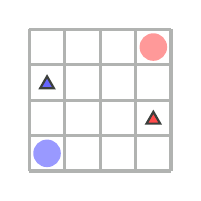
\begin{tikzpicture}[scale=0.45]
                % Grid Lines
                \draw[grigioScuro!40, very thick] (0,0) grid (4,4);
                
                % Bases (Circles)
                \node[circle, fill=blue!40, minimum size=0.35cm] at (0.5,0.5) {};
                \node[circle, fill=red!40, minimum size=0.35cm] at (3.5,3.5) {};
                
                % Agents (Triangles) - FIXED: Smaller size for the grid (minimum size=0.28cm)
                \node[draw=grigioScuro, thick, regular polygon, regular polygon sides=3, fill=blue!60, minimum size=0.2cm, inner sep=0pt] at (0.5,2.45) {};
                \node[draw=grigioScuro, thick, regular polygon, regular polygon sides=3, fill=red!70, minimum size=0.2cm, inner sep=0pt] at (3.5,1.45) {};
            \end{tikzpicture}
            
        \end{column}
        
        % Right Column: Reward Machine Automaton
        \begin{column}{0.35\textwidth}
            \centering
                \begin{center}
                    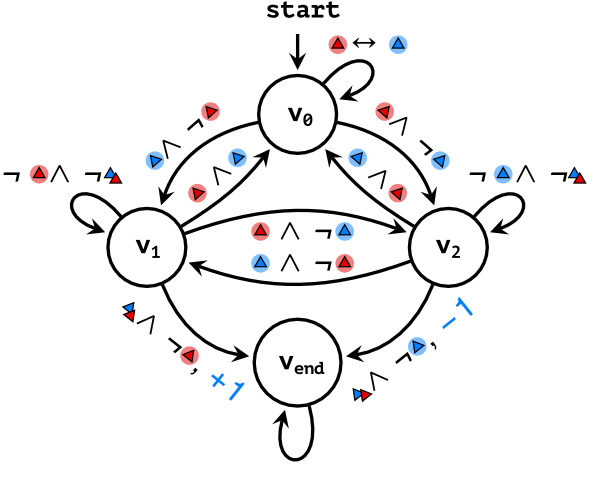
\includegraphics[width=1\textwidth]{images/plotRM.png}
                \end{center}
        \end{column}
        \begin{column}{0.33\textwidth}
            \centering
            $$L(s_t, a_{\mathfrak{a}}, a_{\mathfrak{e}},s_{t+1}) = \{ \redbase, \bluebase \}$$            
        \end{column}
        
    \end{columns}
    \scriptsize{\textbf{Figure}. Example Grid World \quad\quad\quad
     \textbf{Figure}.Example Associated RM  \quad\quad\quad\quad\quad\quad\quad\quad
     \textbf{Equation}. Example Labelling function}
     \hspace*{10.8cm}\scriptsize{output}
\end{frame}


% Slide 9: Augmented State Space Framework
%\begin{frame}{The Augmented State Space Framework}
%    \begin{block}{Labeling Function ($L$)}
%        Maps environment transitions to logical propositions:
%        \[L: S \times A_{\mathfrak{e}} \times A_{\mathfrak{a}} \times S \rightarrow 2^{\mathcal{P}}\]
%        $l_t = L(s_t, a_{\mathfrak{a},t}, a_{\mathfrak{e},t}, s_{t+1})$ is the set of true propositions in $\mathcal{P}$ at step $t$.
%    \end{block}
%    
%    \begin{alertblock}{Lemma 1: Markovian Restoration}
%        The product stochastic game has \textbf{Markovian reward functions} that express the original non-Markovian rewards.
%    \end{alertblock}
%    \begin{itemize}
%        \item Given $l_t$, the RM state transitions to $v_{t+1} = \delta(v_t, l_t)$ and outputs reward $r_{t} = \sigma(v_t, l_t)$.
%        \item This resolves historical dependencies and enables standard Q-learning.
%    \end{itemize}
%\end{frame}

%\section{Game Theory Setting and Problem formulation}
\section{Q-learning with RM for SG}

% Slide 10: Product Stochastic Game


\begin{frame}{Markovian formulation of SG with RMs}
    %The SG with non-markovian reward functions is formalized as \evidenzia{a product stochastic game} to obtain \evidenzia{Markovian rewards} using reward machines.
    %\vspace{0.2cm}

    \begin{block}{Definition | Stochastic Game with Reward Machines (SGRM)}
        \vspace{0.2cm}Given an SG $\mathcal{G}$ and RMs $\mathcal{A}_{\mathfrak{e}}, \mathcal{A}_{\mathfrak{a}}$, a SGRM is defined as a product stochastic game:

        \begin{center}
            $\mathcal{H} = (S', s'_I, A_{\mathfrak{e}}, A_{\mathfrak{a}}, p', R'_{\mathfrak{e}}, R'_{\mathfrak{a}}, \gamma)$
        \end{center}

        \begin{itemize}
            \item \textbf{Augmented State Space:} $S' = S \times V_{\mathfrak{e}} \times V_{\mathfrak{a}}$. An \evidenzia{augmented state} is $s' = (s, v_{\mathfrak{e}}, v_{\mathfrak{a}})$.
            %\item \textbf{Initial Augmented State:} $s'_I = (s_I, v_{I,\mathfrak{e}}, v_{I,\mathfrak{a}})$.
            \item \textbf{Transition Probabilities:} $p'(s', a_{\mathfrak{e}}, a_{\mathfrak{a}}, \bar{s}') = p(s, a_{\mathfrak{e}}, a_{\mathfrak{a}}, \bar{s})$ if $v_i' = \delta_i(v_i, L(s, a_{\mathfrak{e}}, a_{\mathfrak{a}}, \bar{s}))$ for \evidenzia{both} $i \in \{\mathfrak{e}, \mathfrak{a}\}$, and $0$ \evidenzia{otherwise}.
            \item \textbf{Markovian Reward Functions:} $R'_i(s', a_{\mathfrak{e}}, a_{\mathfrak{a}}, \bar{s}') = \sigma_i(v_i, L(s, a_{\mathfrak{e}}, a_{\mathfrak{a}}, \bar{s})),\quad \forall i$
        \end{itemize}
    \end{block}
    \vspace{0.2cm}

\end{frame}


\begin{frame}{Why the SGRM formulation?}

    The newly introduced Stochastic Game $\mathcal{H}$ is proved to have a \evidenzia{Markovian rewards functions} $R'_i$ \evidenzia{which expresses the original} Stochastic Game $\mathcal{G}$ \evidenzia{non-Markovian reward functions} $R_i$ ($\forall i\in\{\mathfrak{e},\mathfrak{a}\}$)

\end{frame}


% \begin{frame}{The Stage Game Matrix}
%     \begin{block}{Definition: Stage Game}
%         A two-player stage game is defined as $(r_\mathfrak{e}, r_\mathfrak{a})$, where $r_i$ is agent i's reward function $R_i$, over the space of joint actions:
%         \[r_i = \{R_i(a_\mathfrak{a}, a_\mathfrak{e}) | a_\mathfrak{a}\in{A_\mathfrak{a}}, a_\mathfrak{e}\in{A_\mathfrak{e}}\} \]
%     \end{block}
%     \begin{itemize}
%         \item In QRM-SG, a stage game is formulated at each time step based on current Q-functions in augmented state space.
%         \item The \textbf{Lemke-Howson method} is used to derive best-response strategies at a Nash equilibrium.
%     \end{itemize}
% \end{frame}

\begin{frame}{SGRM steps in practice}

 \begin{enumerate}
 \item The agent consider $S'$ to select actions:
 \begin{enumerate}
    \item At each time step each agent \evidenzia{selects} the \evidenzia{action to perform in $s$}, \evidenzia{simultaneously} executed.
    \item Action execution causes \evidenzia{game state transition} from $s$ to $s'$. $$s\overset{a_\mathfrak{e},a_\mathfrak{a}\ \ }{\longrightarrow} s'$$
 \end{enumerate}
 \item The tuple ($s_t, a_\mathfrak{e},a_\mathfrak{a},s_{t+1}$) becomes then available.
 \begin{enumerate}
    \item With this input, $L$ returns the \evidenzia{set of satisfied atomic proposition} of $\mathcal{P}$, $l_t$.
    \item Accordingly to available action with $l_t$, a \evidenzia{transition} is performed over each agent RM: 
    $$v_\mathfrak{e}\overset{l_t}{\longrightarrow} v'_\mathfrak{e} \quad v_\mathfrak{a}\overset{l_t}{\longrightarrow} v'_\mathfrak{a}$$
\end{enumerate}

 \item RM transitions lead to each agent reward obtainance: $r_{i,t} = \sigma(v_\mathfrak{i}, L(s, a_\mathfrak{e}, a_\mathfrak{a}, s'))$
\end{enumerate}
\end{frame}


\begin{frame}{Q-functions at Nash Equilibrium}

    In SGRM we define the \evidenzia{optima Q-function} for agent $i$ the...
    \vspace{0.3cm}
    \begin{block}{Q-function at a Nash Equilibrium}
    It is the \evidenzia{EDCR} obtained by agent i when both agents \evidenzia{follow a joint Nash equilibrium strategy} from the next period on. In augmented space $S \times V_{\mathfrak{e}} \times V_{\mathfrak{a}}$ it is defined:
    \[ q_{i}^{*}(s,v_{\mathfrak{e}},v_{\mathfrak{a}},a_{\mathfrak{e}},a_{\mathfrak{a}})=r_{i} + \gamma\sum_{s^{\prime}, v'}p(s^{\prime},v'|s,v,a_{\mathfrak{e}},a_{\mathfrak{a}})\underbrace{\tilde{v}_{i}(s^{\prime},v_{\mathfrak{e}}^{\prime},v_{\mathfrak{a}}^{\prime},\pi_{\mathfrak{e}}^{*},\pi_{\mathfrak{a}}^{*})}_{\substack{\text{Following NE from}\\\text{next period on}}} \]
    
\end{block}
\end{frame}


% Slide 11: Nash Equilibrium & The Stage Game


\begin{frame}{Finding optimal Policies}

    Given the both agent Q-function, \evidenzia{best response policies} are then originally extracted using the \evidenzia{Lemke-Howson method}:
    $$\pi^{NE}_\mathfrak{e}, \pi^{NE}_\mathfrak{a} \leftarrow \textsc{\text{\small lh\_method}}(Q_\mathfrak{e},Q_\mathfrak{a})$$

    ...But an agent is blind to the other Q-function due to adversarial problem nature. 
    
    However, since both receive same signal ($s_t, a_\mathfrak{e},a_\mathfrak{a},s_{t+1}$), using \evidenzia{personal RMs}, they estimate opponents rewards, \evidenzia{estimating opponent Q-Function} too:

    $$\underbrace{Q_{\mathfrak{e},\mathfrak{e}} \quad\quad Q_{\mathfrak{a},\mathfrak{e}}}_{\text{Agent Ego estimations}} \quad\quad \underbrace{Q_{\mathfrak{a},\mathfrak{a}} \quad\quad Q_{\mathfrak{e},\mathfrak{a}}}_{\text{Agent Adv estimations}}$$
% \begin{itemize}
    %     \item $q_{ij}$ represents the Q-function for agent $i$ as learned by agent $j$.
    %     \item Each agent learns the Q-functions of \textbf{all agents} in the system to calculate current equilibria locally.
    % \end{itemize}
\end{frame}

\begin{frame}{Finding optimal Policies (cont'd)}
    

    \begin{block}{Definition: Stage Game}
        A two-player stage game is defined as $(r_\mathfrak{e}, r_\mathfrak{a})$, where $r_i$ is agent i's reward function $R_i$, over the space of joint actions:
        \[r_i = \{R_i(a_\mathfrak{a}, a_\mathfrak{e}) | a_\mathfrak{a}\in{A_\mathfrak{a}}, a_\mathfrak{e}\in{A_\mathfrak{e}}\} \]
    \end{block}
    

    In QRM-SG, a stage game is formulated at each time step based on current Q-functions in augmented state space. 
    
    %Due to the \evidenzia{obtained Markovianity} of SGRM, we're allowed to decompose the problem and \evidenzia{derive best-response strategies at a NE at each step} of each episode.
    Because the product stochastic game with reward machines has Markovian rewards, QRM-SG can apply Nash-Q updates: at each augmented state, it derives a Nash equilibrium of the current Q-value stage game and uses the associated best-response strategies in the Q-function update.
\end{frame}

%\section{Unified Framework}
\section{QSG-RM Algorithm Overview}

% Slide 12: QRM-SG Architecture
\begin{frame}{QRM-SG Algorithm Key aspects}
    \begin{block}{Actor Mechanics (Action Selection)}
        \begin{itemize}
            %\item Balances policy \evidenzia{exploration} and \evidenzia{exploitation} an $\epsilon$-greedy wrapper around calculated stage-game equilibrium solutions.
            \item $\epsilon$-greedy policy is adopted to balance the \evidenzia{exploration} and \evidenzia{exploitation}.
            %\item With probability $1-\epsilon$, the model chooses the max probabiity action in mixed-strategy $\pi_{\mathfrak{e},\mathfrak{e}}$, $\pi_{\mathfrak{a},\mathfrak{a}}$ outputed by \evidenzia{Lemke-Howson algorithm} %tracks the maximum probability mixed-strategy $\pi_{\mathfrak{e},\mathfrak{e}}$, $\pi_{\mathfrak{a},\mathfrak{a}}$ outputed by \evidenzia{Lemke-Howson algorithm}.
            {
            %\footnotesize
            $$a_i \leftarrow 
            \left\{
                \begin{aligned}
                &\operatorname{argmax}_{a\in A_i} \pi_{ii}(a \mid s, v_\mathfrak{e}, v_\mathfrak{a}) && {\footnotesize\text{with probability } 1-\epsilon} \\
                &\text{random} && {\footnotesize\text{with probability } \epsilon}\\
            \end{aligned}
            \right.
            $$
            }
        \end{itemize}
    \end{block}
    \vspace{0.2cm}
    
    \begin{block}{Critic Updates (Learning Loop)}
        Values are updated according to standard stochastic approximation:
        \[ q_{ji} \leftarrow (1-\alpha_{t})q_{ji} + \alpha_{t}(r_{i,t} + \gamma \overline{q}_{ji}(s^{\prime}, v_{\mathfrak{e}}^{\prime}, v_{\mathfrak{a}}^{\prime})) \]
        where %$\overline{q}_{ji}\in \mathbb{R}$ is the expected value at the next augmented state under best-response actions:
        \[ \bar q_{ji} \leftarrow \pi_{\mathfrak{e},\mathfrak{i}}(s', v'_\mathfrak{e}, v'_\mathfrak{a} )  \pi_{\mathfrak{a},\mathfrak{i}}(s', v'_\mathfrak{e}, v'_\mathfrak{a} )  q_{ji} (s', v'_\mathfrak{e}, v'_\mathfrak{a} ) \in \mathbb{R}\]
    \end{block}
\end{frame}

\subsection{Algorithmic Phase Analysis}

\begin{frame}{QRM-SG Phase 1 | Initialization}
    \begin{block}{Process Breakdown (Lines 1--4)}
    \begin{algorithmic}
        \vspace{0.2cm}
        \STATE \textbf{Hyperparameter}: episode length $eplength$, $\gamma$, $\epsilon$
        \STATE \textbf{Input}: Reward machines $\mathcal{A}_{\mathfrak{e}}, \mathcal{A}_{\mathfrak{a}}$
        \vspace{0.2cm}
        %\STATE \textbf{Initialize} $\alpha_t, \gamma, \epsilon$ 
        \STATE $s \leftarrow InitialState(); v_{\mathfrak{e}} \leftarrow v_{I,\mathfrak{e}}; v_{\mathfrak{a}} \leftarrow v_{I,\mathfrak{a}}$ 
        \STATE $q_{\mathfrak{e}i}(\cdot), q_{\mathfrak{a}i}(\cdot) \leftarrow InitialQfunctions()$ 
    \end{algorithmic}
    \end{block}
    \evidenzia{Analysis:}
    \begin{itemize}
        \item Each agent initializes \evidenzia{two} Q-tables to store values for self and opponent, allowing local equilibrium computation. 
        \item SGRM (augmented) states are defined in the product space $S \times V_{\mathfrak{e}} \times V_{\mathfrak{a}}$.%; each tuple element $s$, $v_{\mathfrak{e}}$ and $v_{\mathfrak{a}}$ is \evidenzia{individually initialized}.  %, ensuring the Markov property is preserved. 
    \end{itemize}
\end{frame}

\begin{frame}{QRM-SG Phase 2 | Nash-Action Selection}
    \begin{block}{Process Breakdown (Lines 7--13)}
    \begin{algorithmic}
        \vspace{0.2cm}
        \STATE {\footnotesize \textcolor{gray}{\# for each episode, for each time step $t$:}}
        \STATE $\bar \epsilon \leftarrow GenerateRandomValue(0,1)$
        \IF{$\overline{\epsilon} < \epsilon$} 
            \STATE $a_i \leftarrow ChooseActionRandomly()$ {\footnotesize \textcolor{gray}{\# Acting at random}}
        \ELSE 
            \FOR{$i \in \{\mathfrak{e}, \mathfrak{a}\}$}
                \STATE $\pi_{\mathfrak{e}i}, \pi_{\mathfrak{a}i} \leftarrow {\textbf{CalculateNashEquilibrium}}(q_{\mathfrak{e}i}, q_{\mathfrak{a}i})$ {\footnotesize \textcolor{gray}{\# Get current best strategy}}
                \STATE $a_i \leftarrow \text{argmax } \pi_{ii}(a|s, v_{\mathfrak{e}}, v_{\mathfrak{a}})$  {\footnotesize \textcolor{gray}{\# ... and select action accordingy}}
            \ENDFOR
        \ENDIF
    \end{algorithmic}
    \end{block}
    %\textbf{Analysis:}
    %\begin{itemize}
    %    \item \textbf{Exploration:} Standard $\epsilon$-greedy mechanism balances discovery and optimization.
    Each agent solves a bimatrix stage game using the \evidenzia{LHmethod} to find mixed strategy equilibria.
    %\end{itemize}
\end{frame}

\begin{frame}{QRM-SG Phase 3 | Reward Machine Dynamics}
    %Previously selected step action gets executed:
    \begin{block}{Process Breakdown (Lines 14--18)}
    \vspace{0.2cm}
        \begin{algorithmic}
        \STATE $s' \leftarrow ExecuteAction(s, a_{\mathfrak{e}}, a_{\mathfrak{a}})$ \textcolor{gray}{\footnotesize \textcolor{gray}{\# Agent State transition}}
        \STATE $l_t \leftarrow L(s, a_{\mathfrak{e}}, a_{\mathfrak{a}}, s')$ 
        \FOR{$i \in \{\mathfrak{e}, \mathfrak{a}\}$}
            \STATE $v_i' \leftarrow \delta_i(v_i, l_t); r_{i,t} \leftarrow \sigma_i(v_i, l_t)$ {\footnotesize \textcolor{gray}{\# Game state transition and immediate rewards}}
        \ENDFOR
    
    \end{algorithmic}
    \end{block}
    \vspace{0.3cm}
    %\evidenzia{Analysis:}
    \begin{itemize}
        \item $L$ bridges physical environmental transitions ($s \to s'$) with high level verification ($l_t$), allowing logic task transitions ($v_i\rightarrow v'_i$)
        %detecting high-level environmental events. (e.g., "Agent i did \textcolor{verdeSalvia}{X}"). 
        \item Rewards $r_{i,t}$ are generated by the RM transitions, making them implicitly \evidenzia{history aware}. 
    \end{itemize}
\end{frame}

\begin{frame}{QRM-SG Phase 4 - Nash Q-Learning}

In single agent settings, Q-functions can be updated via the \evidenzia{off policy Q-learning}, with rule: %method can be used to update the Q-function estimation, as a TD learning method, using the following update rule:
    %$$Q(s,a) \leftarrow Q(s,a) + \alpha[r + \gamma \max_{a'} Q(s',a') - Q(s,a)]$$
    $$Q(s,a) \leftarrow Q(s,a) + \alpha[r + \gamma \mathop{\mathbf{\color{black}{max}}}_{a'} Q(s',a') - Q(s,a)]$$
    But not if rewards depend on the joint behavior of more agents. The EDCR averaging w.r.t. policy $\pi$ moves to:
    $$\max_a' Q(s',a') \quad \longrightarrow \quad 
    \mathbb{E}_{\pi_{\mathfrak{e},i},\pi_{\mathfrak{a},i}}[\ Q_{\mathfrak{e},i}(s',a')\ ] $$

    %But the max operator is \evidenzia{not applicable in a multi-agent setting}, where reward depends on joint behavior. This is then sobstituted by the \evidenzia{Nash equilibrium}, for each agent q-function:
    
    Nash-Q-Learning makes use of  co-dependent expectation. Each agent $i$ updates its estimates:
    $$Q_{\mathfrak{e},i} (s,\textbf{a}) \leftarrow Q_{\mathfrak{e},i} (s,\textbf{a}) + \alpha (r_{\mathfrak{e},i} + \gamma \mathbb{E}_{\pi_{\mathfrak{e},i},\pi_{\mathfrak{a},i}} [\ Q_{\mathfrak{e},i}(s',\textbf{a}') \ ] - Q_{\mathfrak{e},i}(s,\textbf{a})\ )$$    
    $$Q_{\mathfrak{a},i} (s,\textbf{a}) \leftarrow Q_{\mathfrak{a},i} (s,\textbf{a}) + \alpha (r_{\mathfrak{a},i} + \gamma \mathbb{E}_{\pi_{\mathfrak{e},i},\pi_{\mathfrak{a},i}} [\ Q_{\mathfrak{a},i}(s',\textbf{a}') \ ] - Q_{\mathfrak{a},i}(s,\textbf{a})\ )$$    

\end{frame}

\begin{frame}{QRM-SG Phase 4 - Nash Q-Learning (cont'd)}

    %$$Nash(Q_i(s',\textbf{a})) = \mathbb{E}_{\textbf{a}} [Q_i(s',\textbf{a})] = \pi_{\mathfrak{e}i}(s', v'_\mathfrak{e}, v'_\mathfrak{a} )  \pi_{\mathfrak{a}i}(s', v'_\mathfrak{e}, v'_\mathfrak{a} )  Q_i (s', v'_\mathfrak{e}, v'_\mathfrak{a} )$$
    Current policies estimations are obtained with a call to \textbf{CalculateNashEquilibrium} function.
    \vspace{0.5cm}

    Compared to classical Q-Learning, the algorithm still looks ahead to the \evidenzia{next state} $(s',v'_\mathfrak{e}, v'_\mathfrak{a})$, but instead of looking at the entry with maximal value wrt action, it \evidenzia{averages with respect to all combinations of agents actions}, weighted by the \evidenzia{joint probability} of action choice.
    
    \vspace{0.5cm}
    
    
\end{frame}

\section{Additional Keypoints}

\begin{frame}{Introduction of the counterfactual Reasoning}

    Original paper Nash Q-learning is as a function of the augmented state space $S \times V_{\mathfrak{e}} \times V_{\mathfrak{a}}$. 
    Additionally, given a state, step update affects only the state $(s, v_{\mathfrak{e}}, v_{\mathfrak{a}})$ after action $a_\mathfrak{e}, a_\mathfrak{a}$.
    
    \vspace{0.5cm}
    \begin{block}{Pointed out problem}
    Given a phisical state $s$, we can reach next $s'$ having \evidenzia{many different} RM internal states $v_\mathfrak{e},v_\mathfrak{a}$. 
    
    Since, the 4 Q-function updates highly depends on $|V_\mathfrak{e}\times V_\mathfrak{a}|$, to perform a \evidenzia{general state game learning}, we would need to \evidenzia{experience a huge amount of steps/episodes}.
    \end{block}

\end{frame}

\begin{frame}{Introduction of the counterfactual Reasoning}

However, \underline{physical states} ($s$) and \underline{logical game states} ($v_\mathfrak{e}, v_\mathfrak{a}$) are \evidenzia{independent}: 
\begin{itemize}
    \item Agents may move in gridworld and receive $l_t$ \evidenzia{regardless of task related history}. 
    \item RM states are meant to keep \evidenzia{only task relevant high-level informations} through $v_i$, \evidenzia{without} \evidenzia{spatial} nor \evidenzia{temporal} informations. 
\end{itemize}
\vspace{0.5cm}
So, during each $s\rightarrow s'$ transition, we can \evidenzia{simulate} having \evidenzia{different RM states}, i.e. simulating \evidenzia{alternative historical backgrounds} at each $s\rightarrow s'$.
\end{frame}

\begin{frame}{Counterfactual Reasoning}
    Instead of needing performing $s\rightarrow s'$ with every possible \evidenzia{history} permutation, we use experience all histories at once.
    \vspace{0.5cm}

    This shifts (\textit{at its best}) complexity \evidenzia{away from exploration} and transfers it into the \evidenzia{computation of an individual trace}.
    
    \vspace{0.5cm}
    \begin{block}{What does it means in practice?}
    For a $N\times M$ grid, 2 agents, 4 actions for agent, RMs with $K_\mathfrak{e}$, $K_\mathfrak{a}$ states, if standard RM based code requires $E$ episodes to converge, then with the counterfactual reasoning we can expect to converge in $\frac{E}{K_\mathfrak{e} \cdot K_\mathfrak{a}}$ episodes.
    \end{block}
\end{frame}

\begin{frame}{Counterfactual Reasoning (cont'd)}

    
    %If an agent enters a cell in which there is a trap, it does even independently from the agent history/memory. 
    %It's the RM, having received the environment label responds \evidenzia{accordingly with the state it is in}.

    \vspace{0.2cm}
    \begin{block}{Counterfactual Reasoning}
    Since the \evidenzia{practical environment transition is independent from the RM state}, instead of updating the Q-value for state $(s, v_{\mathfrak{e}}, v_{\mathfrak{a}})$ \evidenzia{only}, we can
    \begin{itemize}
        \item Consider all RMs states $\tilde v_{\mathfrak{e}},\tilde v_{\mathfrak{a}}$, simulate being in augmented state $(s, \tilde v_{\mathfrak{e}},\tilde v_{\mathfrak{a}})$.
        \item Simulate state and the RM transition to $\tilde v'_{\mathfrak{e}},\tilde v'_{\mathfrak{a}}$ if $s'$ is reached, i.e. reaching $(s', \tilde v'_{\mathfrak{e}},\tilde v'_{\mathfrak{a}})$
        \item Update  the Q-function associated to $(s, \tilde v_{\mathfrak{e}},\tilde v_{\mathfrak{a}})$
    \end{itemize} 
    \end{block}

\end{frame}


\begin{frame}{Convergence Assumptions}
    \begin{block}{Assumption 1: Exploration}
        Every state $s \in S$, RM states $v_{\mathfrak{e}} \in V_{\mathfrak{e}}$, $v_{\mathfrak{a}} \in V_{\mathfrak{a}}$, and actions $a_{\mathfrak{e}} \in A_{\mathfrak{e}}$, $a_{\mathfrak{a}} \in A_{\mathfrak{a}}$, are visited infinitely often when the number of episodes goes to infinity. 
    \end{block}
    \vspace{0.2cm}

    \begin{block}{Assumption 2: Learning Rate}
        The learning rate $\alpha_t$ satisfies the following conditions for all $t$:
        \begin{enumerate}
            \item $0 < \alpha_t < 1$, $\sum_t \alpha_t(s, v_{\mathfrak{e}}, v_{\mathfrak{a}}, a_{\mathfrak{e}}, a_{\mathfrak{a}}) = \infty$, $\sum_t [\alpha_t(s, v_{\mathfrak{e}}, v_{\mathfrak{a}}, a_{\mathfrak{e}}, a_{\mathfrak{a}})]^2 < \infty$, and the latter two hold uniformly and with probability 1. 
            \item $\alpha_t(s, v_{\mathfrak{e}}, v_{\mathfrak{a}}, a_{\mathfrak{e}}, a_{\mathfrak{a}}) = 0$ if $(s, v_{\mathfrak{e}}, v_{\mathfrak{a}}, a_{\mathfrak{e}}, a_{\mathfrak{a}}) \neq (s^t, v_{\mathfrak{e}}^t, v_{\mathfrak{a}}^t, a_{\mathfrak{e}}^t, a_{\mathfrak{a}}^t)$.
        \end{enumerate}
    \end{block}
\end{frame}

\begin{frame}{Convergence Assumptions}
    \begin{block}{Assumption 3: Stage Game Structure}
        One of the following conditions holds during learning: 
        \begin{enumerate}
            \item Every stage game $(q_{\mathfrak{e}i}(s, v_{\mathfrak{e}}, v_{\mathfrak{a}}), q_{\mathfrak{a}i}(s, v_{\mathfrak{e}}, v_{\mathfrak{a}}))$, $i \in \{\mathfrak{e}, \mathfrak{a}\}$, for all $t, s, v_{\mathfrak{e}}, v_{\mathfrak{a}}$, has a \evidenzia{\underline{global} optimal point} $(\tilde{\pi}_{\mathfrak{e}i}, \tilde{\pi}_{\mathfrak{a}i})$ (i.e., $\tilde{\pi}_{ji}q_{ji} \geq \tilde{\pi}_{ji}'q_{ji}$ for any $\tilde{\pi}_{ji}'$, $j \in \{\mathfrak{e}, \mathfrak{a}\}$) and agents' rewards in this equilibrium are used to update their Q-functions. 
            \item Every stage game $(q_{\mathfrak{e}i}(s, v_{\mathfrak{e}}, v_{\mathfrak{a}}), q_{\mathfrak{a}i}(s, v_{\mathfrak{e}}, v_{\mathfrak{a}}))$, $i \in \{\mathfrak{e}, \mathfrak{a}\}$, for all $t, s, v_{\mathfrak{e}}, v_{\mathfrak{a}}$, has a \evidenzia{\underline{saddle} point} $(\tilde{\pi}_{\mathfrak{e}i}, \tilde{\pi}_{\mathfrak{a}i})$ (i.e., $\tilde{\pi}_{ji}\tilde{\pi}_{-ji}q_{ji} \geq \tilde{\pi}_{ji}'\tilde{\pi}_{-ji}q_{ji}$ for any $\tilde{\pi}_{ji}'$, $\tilde{\pi}_{ji}\tilde{\pi}_{-ji}q_{ji} \leq \tilde{\pi}_{ji}\tilde{\pi}_{-ji}'q_{ji}$ for any $\tilde{\pi}_{-ji}'$, $j \in \{\mathfrak{e}, \mathfrak{a}\}$), and agents' rewards in this equilibrium are used to update their Q-functions. 
        \end{enumerate}
    \end{block}


\end{frame}

% \begin{frame}{Theorem 1: Convergence Guarantee}
%     \begin{block}{Theorem 1}
%         Under Assumptions 1, 2 and 3, the sequence $q_{it}=(q_{\mathfrak{e}i}^t, q_{\mathfrak{a}i}^t)$ at time $t$, $i \in \{\mathfrak{e}, \mathfrak{a}\}$ updated by: 
%         \begin{equation*}
%         \begin{aligned}
%             q_{ji}(s, v, a) = &(1-\alpha_t)q_{ji}(s, v, a) + \\ 
%             &\alpha_t(r_{j,t} + \gamma \pi_{\mathfrak{e}i}(\cdot | s', v')\pi_{\mathfrak{a}i}(\cdot | s', v')q_{ji}(s', v'))
%         \end{aligned}
%         \end{equation*} 
%         for $j \in \{\mathfrak{e}, \mathfrak{a}\}$, where $(\pi_{\mathfrak{e}i}(\cdot|s', v'), \pi_{\mathfrak{a}i}(\cdot|s', v'))$ is the appropriate type of Nash equilibrium solution for the stage game $(q_{\mathfrak{e}i}^t(s', v'), q_{\mathfrak{a}i}^t(s', v'))$, converges to the Q-functions at a Nash equilibrium $(q_{\mathfrak{e}i}^*, q_{\mathfrak{a}i}^*)$.
%     \end{block}
% \end{frame}

% Slide 17: Algorithm 1: QRM-SG Pseudocode
% \begin{frame}{Algorithm 1: QRM-SG Full Pseudocode}
%     \begin{algorithmic}[1]
%         \STATE \textbf{Initialize} $q_{\mathfrak{e}i}$ and $q_{\mathfrak{a}i}$ for all $i \in \{\mathfrak{e}, \mathfrak{a}\}$
%         \FOR{episode $l=1,2,\dots$}
%             \STATE $s \leftarrow s_I, v_{\mathfrak{e}} \leftarrow v_{I,\mathfrak{e}}, v_{\mathfrak{a}} \leftarrow v_{I,\mathfrak{a}}$
%             \FOR{$t=0$ \textbf{to} $eplength$}
%                 \STATE Choose action $a_i$ using $\epsilon$-greedy policy and \textbf{Lemke-Howson}
%                 \STATE Execute actions, observe $s'$, and high-level event $l_t = L(s, a_{\mathfrak{e}}, a_{\mathfrak{a}}, s')$
%                 \STATE Update RM states: $v_i' \leftarrow \delta_i(v_i, l_t)$ and reward $r_{i,t} \leftarrow \sigma_i(v_i, l_t)$
%                 \STATE Compute Nash strategy $\pi_{ji}(\cdot|s', v')$ at next augmented state
%                 \STATE Update Q-functions:
%                 \STATE $q_{ji} \leftarrow (1-\alpha_t)q_{ji} + \alpha_t(r_{j,t} + \gamma \sum \pi \pi q_{ji}')$
%                 \STATE $s \leftarrow s', v_{\mathfrak{e}} \leftarrow v_{\mathfrak{e}}', v_{\mathfrak{a}} \leftarrow v_{\mathfrak{a}}'$
%             \ENDFOR
%         \ENDFOR
%     \end{algorithmic}
% \end{frame}

% Slide 18: Algorithm Analysis
% \begin{frame}{Algorithm Analysis and Convergence Properties}
%     \begin{itemize}
%         \item \textbf{Off-Policy Learning:} RMs enable decomposition of complex RL problems into structured subproblems for efficient learning.
%         \item \textbf{Coupled Learning:} The learning processes of agents are coupled because the high-level events depend on joint actions.
%         \item \textbf{Decentralized View:} Each agent maintains a "centralized" perspective by learning everyone's Q-functions to compute equilibria locally.
%     \end{itemize}
% \end{frame}

% % Slide 20: Mathematical Foundation: Convergence Proof
% \begin{frame}{Mathematical Foundation: Convergence Proof}
%     The proof relies on viewing the update as a stochastic approximation of a mapping $F^t$: 
%     \begin{block}{Key Lemmas from Supplementary Materials}
%         \begin{itemize}
%             \item \textbf{Lemma 2:} Establishes general convergence for iterations $q^{t+1}=(1-\alpha_t)q^t + \alpha_t[F^tq^t]$.
%             \item \textbf{Lemma 4:} Shows that Q-functions at a Nash equilibrium ($q^*$) are fixed points of $F^t$, i.e., $q^* = \mathbb{E}[F^t q^*]$.
%             \item \textbf{Lemma 7:} Proves $F^t$ is a \textbf{contraction mapping} under Assumption 3:
%             \[ ||F^t q - F^t \dot{q}|| \le \gamma ||q - \dot{q}|| \]
%         \end{itemize}
%     \end{block}
% \end{frame}

\section{Game Results and Experiments}

% Slide 21: Experimental Framework & Baselines
\begin{frame}{Experimental Framework \& Baselines}
    
        \textbf{Testing Environment:} Evaluated on $6\times6$ (and $12\times12$) competitive, sparse-reward grid world variations of Pac-Man.
        
        \vspace{0.2cm}
        \textbf{Comparative Baselines:}
        \begin{itemize}
            \item \texttt{Nash-Q}: Pure spatial state-action tracking.
            %\item \texttt{Nash-QAS}: Incorporates an unstructured history status vector.
            %\item \texttt{MADDPG-SG} \& \texttt{MADDPG-AS}: Deep multi-agent deterministic policy gradient variants.
        \end{itemize}
\end{frame}

% Slide 22: Empirical Performance
\begin{frame}{Case Study Empirical Analysis}
    \begin{itemize}
        \item \textbf{Case Study I (Sequential Ordering):} QRM-SG converges to equilibrium by $\approx 7,500$ episodes, whereas unaugmented baselines fail entirely.
        \item \textbf{Case Study II \& III (Energy Loops):} Explores complex recharge loops with randomized origin points. QRM-SG reaches stability within $\approx 1,000$ to $1,500$ runs.
        \item \textbf{Scalability:} Successfully finds the Nash equilibrium on an expanded $12\times12$ map space by episode 21,000.
    \end{itemize}
\end{frame}

\section{Conclusion}

% Slide 23: Summary
\begin{frame}{Summary \& Future Outlook}
    \begin{itemize}
        \item \textbf{Core Contribution:} Bridges reward machines with MARL to model non-Markovian constraints in stochastic games.
        \item \textbf{Robust Architecture:} Augmented state transformations allow tabular actors to navigate complex environments successfully.
        \item \textbf{Future Directions:} Dynamically learning unknown reward machine configurations simultaneously during policy calculation; extensions to general-sum games with more agents.
    \end{itemize}
\end{frame}

\section{References}
\begin{frame}[allowframebreaks]{References}
    \setbeamertemplate{bibliography item}[text] % Forza Beamer a mostrare i numeri [1] al posto dei loghi dei libri
    \bibliographystyle{plain} % 'plain' assegna i numeri progressivi [1], [2], ecc.
    \bibliography{references}
\end{frame}

\end{document}